\documentclass[12pt,a4paper]{article}

\usepackage{geometry}
 \geometry{
 a4paper,
 total={170mm,257mm},
 left=20mm,
 top=20mm,
 }
 
\usepackage[english]{babel}
\usepackage[utf8]{inputenc}
\usepackage{amsmath}
\usepackage{amsfonts}
\usepackage{bm}
%\usepackage {natbib}
\usepackage{graphicx,caption,subcaption,float}

\usepackage[colorlinks=true,
            linkcolor=red,
            urlcolor=blue,
            citecolor=blue]{hyperref}

\title{\Huge Time Series Analysis in  Python}

\author{Wenyan Gong, Zongxi Li, Cong Ma, \\
Qingcan Wang, Zhuoran Yang, Hao Zhang}

\date{\today}

\begin{document}
\maketitle

\section{Project Objective}
Time series analysis comprises methods for analyzing time series data in order to extract meaningful statistics and other characteristics of the data. It is widely used in signal processing, pattern recognition, mathematical finance, weather forecasting, earthquake prediction, control engineering, and largely in any domain of applied science and engineering which involves temporal measurements. As in Figure \ref{fig:time_series}, we plot the USD to CNY exchange rate.

In this project, we will play a game with time series in finance. It has gained its popularity in Wall Street recently, since it is fundamental to most promising quantitative investment strategies. We develop a system that can predict future prices of stocks using various kinds of methods for time series analysis. 

\begin{figure}[H]
        \centering
     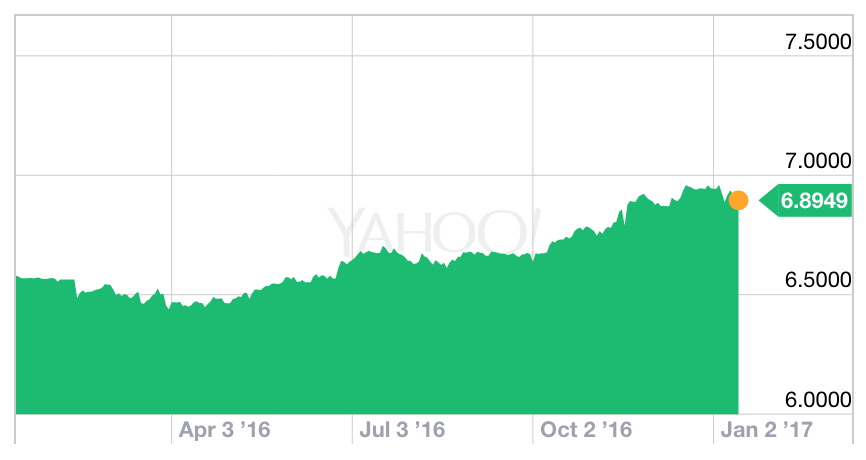
\includegraphics[width=.7\linewidth]{./Figure/USD-CNY.png}
\caption{USD to CNY exchange rate. Jan 12 2016 - Jan 12 2017. Source, Yahoo finance.}
\label{fig:time_series}
\end{figure}

Given input of a stock price series, our system will first fit some powerful and popular time series models, such as the autoregressive (AR) model and the moving average (MA) model. This procedure will give you the estimator of the parameters in these models. 

The most important ingredient in estimation is the optimization procedure. Users can select one of optimization methods in the system based on their preference. The optimization method includes but not limited to gradient descent and gradient descent with momentum.

After model fitting and estimation, our system provides a fast way to do statistical inference. Users can do different kinds of statistical test as well as obtain confidence intervals. Moreover, with fitted model, future price prediction is made and it’s compared with real price data. Moreover, we provide different methods to assess the prediction accuracy, which will be visualized afterwards. With the identified model, we can further consider trading strategy and option pricing.

More interestingly, if users input multiple stock prices, we can divide these stocks into different groups, which is called clustering. Among each group, stocks share certain degree of similarity. Different clusters will also be visualized. With collection of stocks (e.g., S\&P 500), we can exploit the correlations within them and build a reduced order model for price prediction. For example, principal component analysis can be used to extract dominant features in the financial market.

\section{Design Process}
Given the tasks, there are many factors to consider. First, we need to specify the programming language to use. We decide to use python, since it's free, and widely distributed. Moreover, there are many powerful packages, e.g., \texttt{numpy} (linear algebra), \texttt{scipy} (scientific computation), \texttt{matplotlib} (plotting library), etc.

We make use of existing packages like \texttt{numpy} and \texttt{matplotlib}, but largely other parts are made by our group. For instance, we implemented various optimization methods like the (stochastic) gradient descent (GD), and GD with momentum.

\texttt{Github} is used to track the progress of this project, and streamlines the collaboration within our group. \texttt{Github} is a powerful and convenient tool that really makes a difference in group development of codes.

We make use of \texttt{Doxygen} to generate documentation for our project. The users can view various classes of this project in an interactive way via a web browser.

\begin{figure}[H]
        \centering
     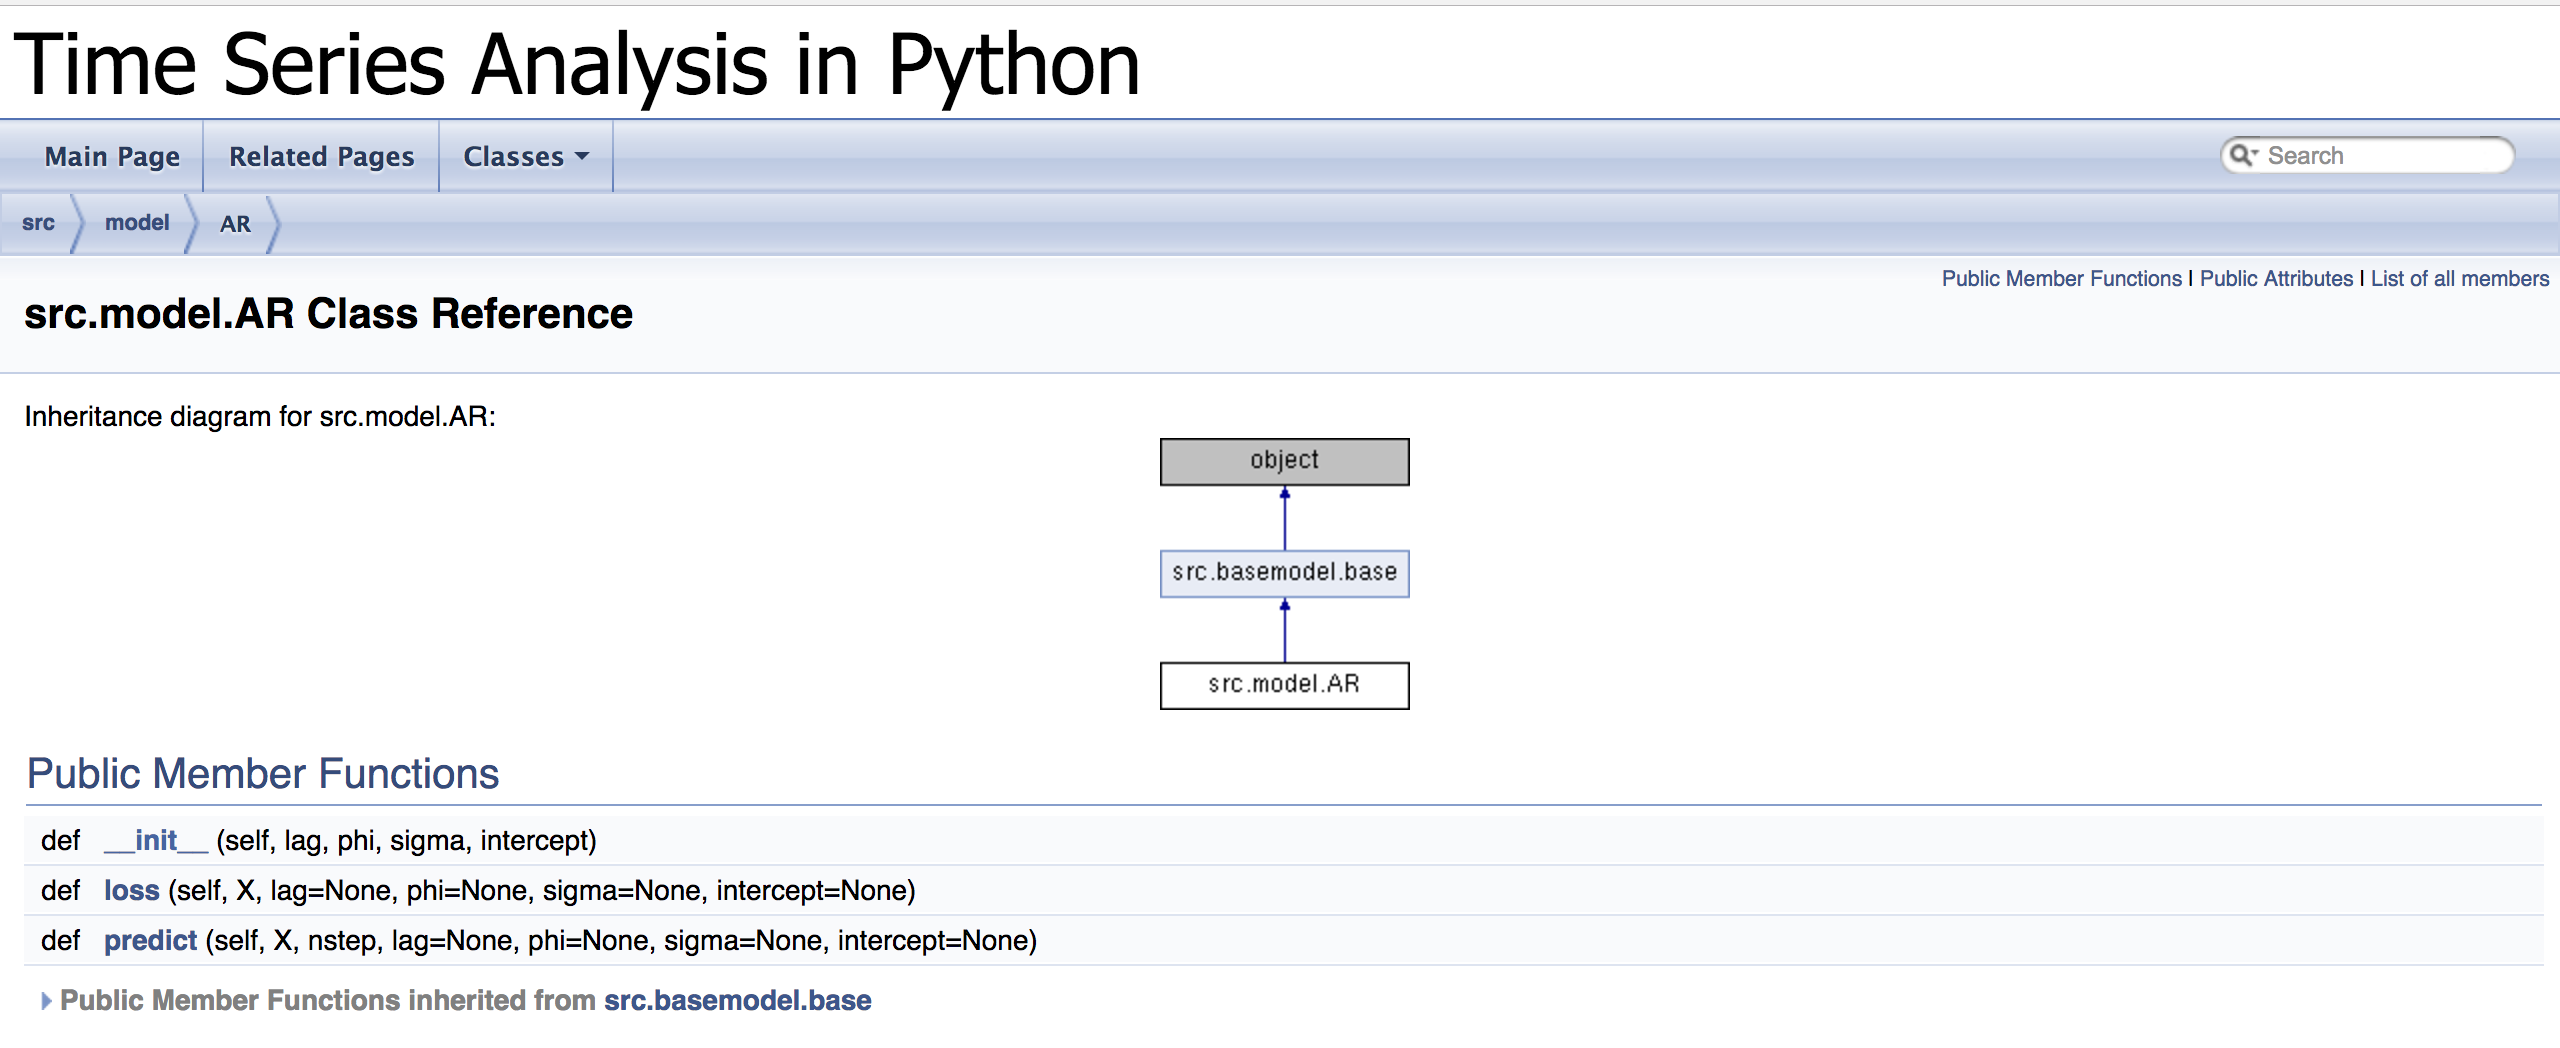
\includegraphics[width=.8\linewidth]{./Figure/Doxygen.png}
\caption{Doxygen documentation}
\end{figure}

Along the way, we have adopted the philosophy of object oriented programming (OOP) by carefully designing classes which include relevant functions. For instance, in the Reduction class, we implemented various model reduction methods including principal component analysis, independent component analysis, and dynamic mode decomposition.

Part of our code are tested using Python unittest, since there are analytical solutions. For more complicated functions, they are tested using canonical examples, and by comparing with the outputs of standard machine learning package scikit-learn.

We have a few milestones for this project. (1) Prototype, Dec 15. In this release, we had at least one implementation for each step. Then given a time series data, we could apply at least one method from each class to do the analysis. (2) Alpha version, Jan 1. In this release, we completed most methods in each class. (3) Final version, Jan 12.  In this release, we finalized the project. Finish all the testing using various data including simulated data and real financial data.

\section{Architecture}
The high-level program structure is shown below. The division of work is pretty even, and there are some minor work that are too trivial to mention extensively here. 
\begin{figure}[H]
        \centering
     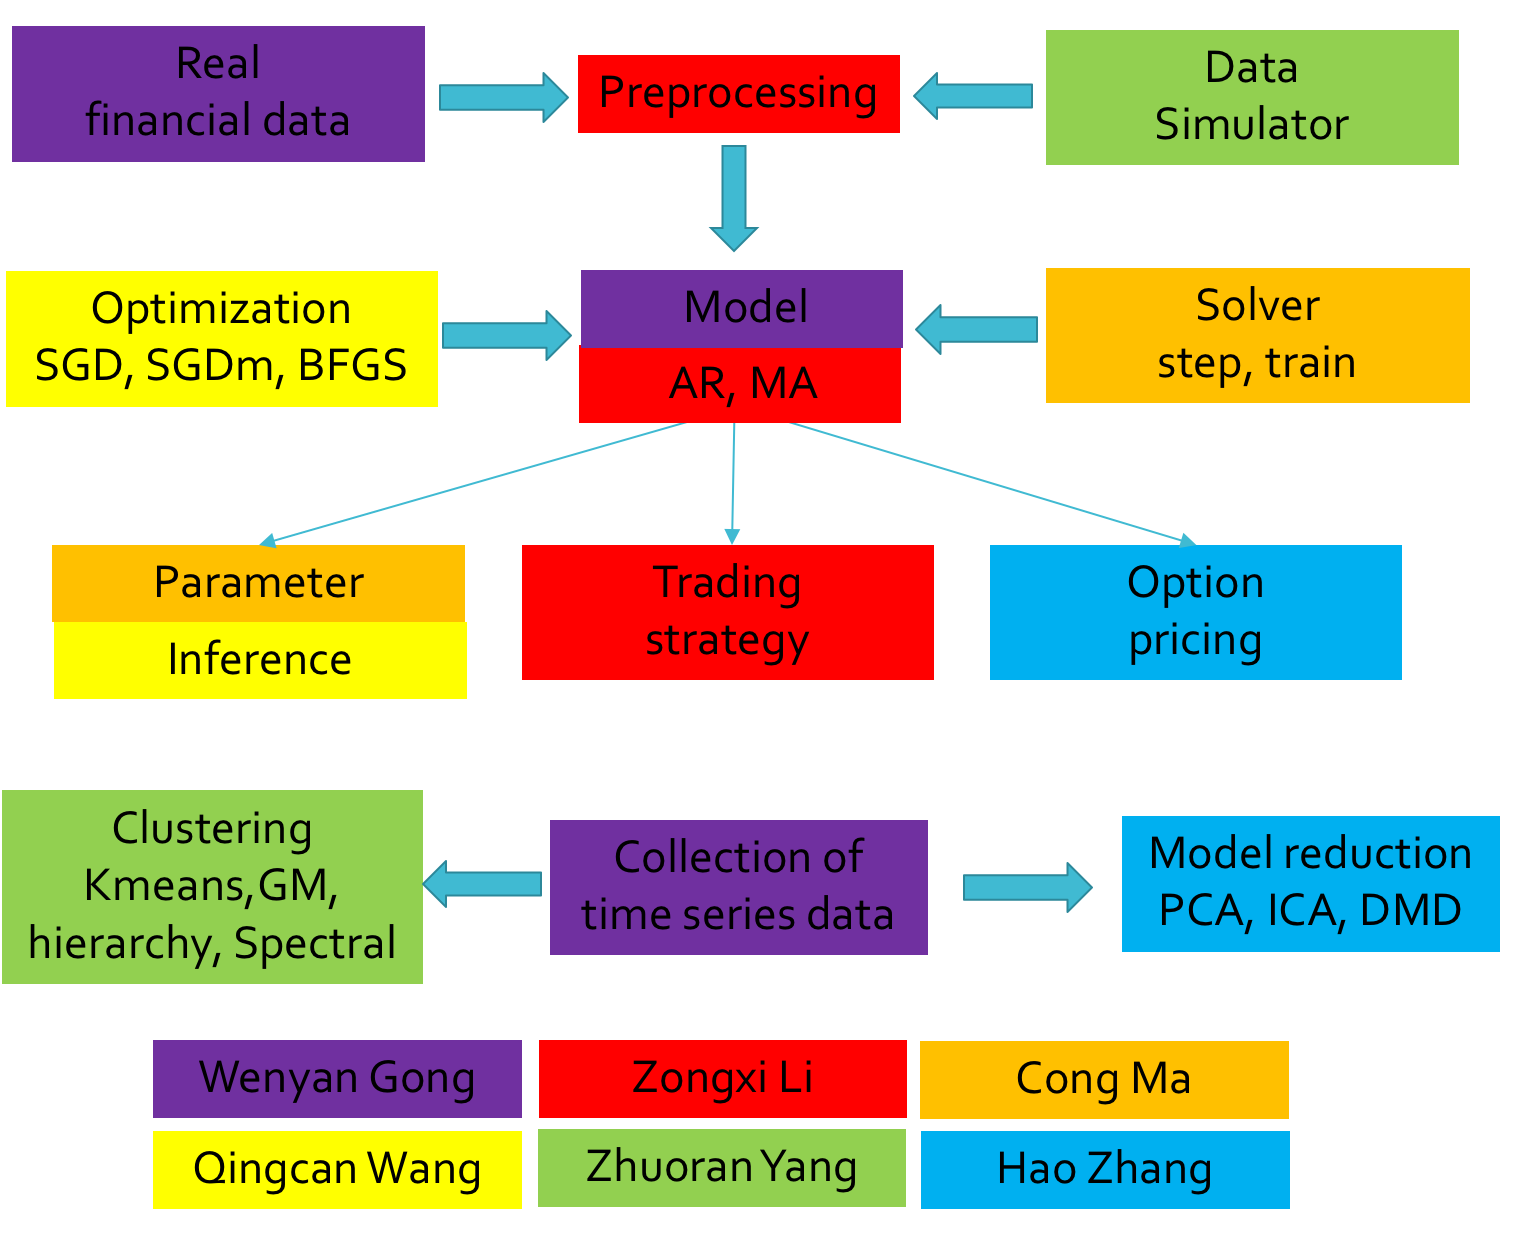
\includegraphics[width=.7\linewidth]{./Figure/structure.png}
\caption{Program structure and division of work}
\end{figure}
Overall, the program consists of two parts. The first part deal with a single time series, and exploits the time correlation within the time series. There is data preprocessing module that takes the raw data and get the right data format for later analysis. Optimization, model, and solver are used all together to identify the models. Finally, there is a post processing module that makes use of the information from model. The post processing module includes parameter inference, trading strategy, and option pricing. The second part deals with a collection of time series of data, basically it exploits the correlation between different time series. In this way, we can gain more insights into the financial market. While these insights are impossible for a single time series.

 
%!TEX root = ../../report.tex
 
 
 
%!TEX root = ../../report.tex

\subsection{Data Preparation and  Preprocessing}

In this package, we provide methods to simulate data from specified time series models and a real-world dataset, thus enabling both theoretical research and applications. 

For simulated data, we provide functions that samples from the \texttt{AR(p), MA(q), ARMA (p,q), GARCH(p,q)} models. Given the parameters of the model, we obtain a $n\times T$ matrix storing  $n$ independent realizations of the time series with time $T$. Since the \texttt{for} loop in \texttt{Python}
is slow, we integrate \texttt{c} code with python using \texttt{Cython}.

For real data, we  provide \texttt{S\&P 500} dataset, which consists of the prices of the Standard \& Poor stocks in a consecutive $490$ days.  In addition, we also  preprocess the raw data, thus enabling users to directly apply various methods on the dataset. More specifically, we provide functions that can transfer the price time series to return time series and do the reverse transferring. For instance, if the user inputs daily price of \texttt{Google} stock, then we can output the daily return of \texttt{Google} stock. If the user inputs the daily return,  we are able to output the daily price. Moreover, we can detect the peak and trough for a given time series, which will be used for developing trading strategy. For example, if you input \texttt{Google} stock price series, we can detect the highest price and the lowest price as well as their location in the time series.

\subsection{Model}
For a given time series, there are two kinds of model class that can be used to fit the time series. One is the autoregressive  (AR) model. The other is the moving average (MA) model. For details, see \cite{Fan}. Inside each class, we provide three functions, initialization, loss function and prediction function. 

To be specific, we can first initialize the model with given parameters. Secondly, the loss function is able to calculate the current loss as well as the gradient of negative loglikelihood function, based on the current parameters in the model. This is crucial, because the loss and gradient will be the input of the optimization method, which will in turn return the updated parameters to the model to calculate new loss and gradient. Finally, the prediction function is able to predict the future time series based on historical time series and fitted parameters.
\subsection{Optimization}
%!TEX root = ../../manual.tex

The optimization part \texttt{optim.py} implements various optimization update
rules: stochastic gradient descent (\texttt{sgd}), stochastic gradient descent
with momentum update (\texttt{sgd\_momentum}) and
Broyden–Fletcher–Goldfarb–Shanno algorithm (\texttt{bfgs}). 

Each update rule accepts current iteration point and the gradient of the object
function and produces the next iteration point. Each update rule has the same
interface:
\begin{lstlisting}[language=Python]
def update(x, dx, config=None):
\end{lstlisting}
The inputs are as follows:
\begin{enumerate}
  \item \texttt{x}:
    A \texttt{numpy} array giving the current iteration point.
  \item \texttt{dx}:
    A \texttt{numpy} array of the same shape as \texttt{x} giving the gradient
    of the object function with respect to \texttt{x}.
  \item \texttt{config}:
    A dictionary containing hyper-parameter values such as learning rate,
    momentum, etc. If the update rule requires caching values over many
    iterations, then config will also hold these cached values.
\end{enumerate}
The outputs are as follows:
\begin{enumerate}
  \item \texttt{next\_x}:
    The next point after the update.
  \item \texttt{config}:
    The config dictionary to be passed to the next iteration of the update rule.
\end{enumerate}

The update rules are called in \texttt{Solver} class like this:
\begin{lstlisting}[language=Python]
objfcn, grads = self.model.objfcn(self.X)
for p, x in self.model.params.iteritems():
    dx = grads[p]
    config = self.optim_configs[p]
    next_x, next_config = self.update_rule(x, dx, config)
    self.model.params[p] = next_x
    self.optim_configs[p] = next_config
\end{lstlisting}




\subsection{Solver}
%!TEX root = ../../report.tex
We develop a solver class, which serves as a bridge between the model class and the optimization methods. Specifically, given the loss function and the gradient functions specified by the model and the optimization methods, the solver uses this method to minimize the loss until it converges. 

\subsection{Inference}
%!TEX root = ../../report.tex

In addition to parameter estimation, we also provide inferential methods that enables users to access the uncertainty of the estimated model. After all, once the model is estimated, it is still not clear how reliable our estimation is. In fact, even for the pure white noise, it is possible to estimate a statistical model, even though that model is not meaningful. 

In specific, we provide functions that estimates the auto-covariance auto-correlation functions (ACF) and perform  the Box-Ljung test  that checks if the  ACF is significant. See \cite{Fan} for a more systematic treatments of statistical inference for time series models. In addition, we provide functions that select the order of \texttt{AR(p)} models, estimate  the parameters, and test whether the parameters are significant.



\subsection{Trading Strategy}

The software is able to generate trading signal based on predicted price. To be specific, it can detect which time point to buy and which to sell. Please see function \texttt{signal\_generation()}. Moreover, it can calculate the profit and loss based on existing trading signal, which can be realized by \texttt{profit\_loss()}

The most important function for the trading is \texttt{rolltrade()} , which can automatically do the trading with historical data and fitted model. This function will call other  functions from the ``model" as well as the functions that generate signals and calculate the profit. It will finally return the predicted price, trading signal and profit time series. Moreover, there are many options for the trading, for instance, you can specify the trading frequency, the prediction length and the initial wealth. 

\subsection{Option Pricing}
%!TEX root = ../../manual.tex

The class \texttt{OptionPricing} calculates the call option price of an underlying
stock based on the Black-Scholes model.

The following parameters are needed to construct an instance of the
\texttt{OptionPricing} class:
\begin{enumerate}
  \item \texttt{sigma}:
    the volatility of the underlying stock price, which is the standard
    deviation of the stock's returns.
  \item \texttt{K}:
    the strike price of the option.
  \item \texttt{T}:
    the expiry time of the option.
  \item \texttt{r}:
    the risk-free interest rate.
  \item \texttt{Smax}:
    the maximum stock price we want to consider.
\end{enumerate}

The method \texttt{solve\_black\_scholes} calculates the option pricing of an
instance, given the grid size of price and time (\texttt{nS} and \texttt{nt}) as
input parameters. The option price as an function of stock price and time will
be stored in the instance.

After running \texttt{solve\_black\_scholes}, we can use 
\texttt{get\_option\_price} method to get the option price of given underlying
stock price \texttt{S} and time \texttt{t}.

Following is a usage example of the \texttt{OptionPricing} class:
\begin{lstlisting}[language=Python]
goog = np.genfromtxt("../data/GOOG.csv", delimiter=",")
sigma = np.std((goog[1:] - goog[:-1]) / goog[:-1])

option_price = OptionPricing(sigma=sigma, T=90, K=800, r=0.005, Smax=1200)
option_price.solve_black_scholes(nS=100, nt=300)
print(option_price.get_option_price(S=810, t=30))
\end{lstlisting}



%!TEX root = ../../report.tex

\subsection{Clustering}
In order to handle the cope with heterogeneous datasets, i.e., datasets with various  characteristics, we provide clustering methods that enable users to perform data analysis with more accuracy.  By utilizing clustering tools, users may discover hidden structures shared by a small subgroup of the dataset  that are buried due to the large scale of the hole dataset. 

To better understand the importance of clustering, let us consider the example of stock market, which consists of stocks that  belong to various sectors. Although there is a global trend of the market as a whole, various sectors may exhibit  different, even converse movements. Thus, global information can be too crude to perform more fine-grained analysis; it would cause huge error if the user predicts the trend of energy stocks using data coming from the whole market.

In the package, we provide a variety of commonly used clustering methods, which include k-means, hierarchical clustering,  spectral clustering, and Gaussian mixture modeling. See   \cite{elsbook} and \cite{bishop2006pattern} for introduction of clustering methods. Our methods yield results  comparable with other machine learning packages in \texttt{python}. In specific, in \texttt{demo\_clustering.ipynb} we showcase our method and  compare with the \texttt{Scikit-Learn} package using the \texttt{S\&P 500} dataset, which consists of the prices of $470$ stocks in a period of $490$ days. A concise illustration is provided in the next section.

\subsection{Model Reduction}
In order to exploit the correlation between various stocks, we develop a model reduction module. As we know, tech companies are expected to have the same stock price trend. Google and Apple might have the same long term behavior. If we view the stock prices at a given time instant as a vector, then as time progresses, the vector changes with time. Principal component analysis (PCA) \cite{jolliffe2002principal} finds dominant structures in the stock market, and the principal component provides a good basis for low dimensional description. Independent component analysis (ICA)\cite{hyvarinen2000independent}  finds the hidden independent signals that generate the stock data. The hidden signals are independent in the sense that they are most non-gaussian. Dynamic mode decomposition (DMD) \cite{jolliffe2002principal}\cite{rowley2009spectral} fits a linear model that transfers the current state to the next state. Given this linear operator (a matrix), we can find its eigenvectors (DMD modes) and eigenvalues (DMD eigenvalues). If we project the initial condition onto leading DMD modes, then each mode evolves with a given frequency (DMD eigenvalue), and this gives the temporal evolution of states.

\section{Demos of results}
\subsection{Modal validation}
%!TEX root = ../../report.tex

To illustrate our clustering methods, we apply our methods on the \texttt{S\&P 500} dataset and compare  with clustering methods provided in the \texttt{Scikit-Learn} package.  We set the number of clusters to $5$ and record the amount of time needed for each of the methods, which is reported in Table-\ref{tab:cluster}. In addition, to visualize the clustering results, we plot all the $470$ stocks with  labels in different colors.  As shown in Figures \ref{fig:cluster1}--\ref{fig:cluster3}, our methods are comparable with  \texttt{Scikit-Learn}.

\begin{table}[htb]
\begin{center}
\begin{tabular}{|c|c|c|c|}
\hline
& K-means &Spectral Clustering & Hierarchical Clustering \\\hline
Our Package & 0.4423 s &0.4749 s& 0.1838 s   \\\hline
\texttt{Scikit-Learn} &0.1308 s & 0.4022 s & 0.1288 s\\\hline
\end{tabular}
\end{center}
\caption{Running time of Clustering Algorithms implemented by our package and \texttt{Scikit-Learn}. As shown in the table, our package provide comparable implementations}
\label{tab:cluster}
\end{table}%

\begin{figure}[htb]
\centering
\hskip-27pt\includegraphics[width=0.5\textwidth]{./Figure/k-means.pdf}
\hskip-12pt\includegraphics[width=0.5\textwidth]{./Figure/SK-k-means.pdf}\\
\caption{K-means clustering for the \texttt{S\&P 500} dataset using our package and   \texttt{Scikit-Learn}.The plot of our clustering result is on the left.}
\label{fig:cluster1}
\end{figure}

\begin{figure}[htb]
\centering
\hskip-27pt\includegraphics[width=0.5\textwidth]{./Figure/SC.pdf}
\hskip-12pt\includegraphics[width=0.5\textwidth]{./Figure/SK-SC.pdf}\\
\caption{Spectral clustering for the \texttt{S\&P 500} dataset using our package and   \texttt{Scikit-Learn}. The plot of our clustering result is on the left.}
\label{fig:cluster2}
\end{figure}

\begin{figure}[htb]
\centering
\hskip-27pt\includegraphics[width=0.5\textwidth]{./Figure/HC.pdf}
\hskip-12pt\includegraphics[width=0.5\textwidth]{./Figure/SK-HC.pdf}\\
\caption{Hierarchical clustering for the \texttt{S\&P 500} dataset using our package and   \texttt{Scikit-Learn}. The plot of our clustering result is on the left.}
\label{fig:cluster3}
\end{figure}

\subsection{Financial data}
With our package, we would be able to play with real financial data: to fit a suitable model and make highly reasonable predictions. In this section, we take the stock return of Google from year 2015-2016 as an example. There are altogether 490 trading days during the time. The stock prices and returns are shown below:

\begin{figure}[H]
        \centering
     \includegraphics[width=.45\linewidth]{./Figure/price.pdf}
     \includegraphics[width=.45\linewidth]{./Figure/return.pdf}
\caption{Left, Google stock pirce. Right, Google stock return.}
\end{figure}

We may fit an \texttt{AR(5)}  model according to the return in the first 480 trading days. Here, the lag value is picked in a moderate size to balance the complexity and validity. By choosing the optimization method to be stochastic gradient descent with momentum update, a fitted model is quickly returned. With the fitted model, we would be able to predict the future return as well as the future stock price for the following days. Here, we make a prediction for 5 days.
\begin{figure}[H]
        \centering
     \includegraphics[width=.45\linewidth]{./Figure/predprice.pdf}
     \includegraphics[width=.45\linewidth]{./Figure/predreturn.pdf}
\caption{Left, predicted Google stock price. Right, predicted Google stock return.}
\end{figure}
As we can see from the figure, we correctly predict the trend of the stock price. Moreover, the predicted price and the true price are very close. This lays a good foundation for the following trading section.

\subsection{Trading strategy}
%!TEX root = ../../report.tex

To illustrate our clustering methods, we apply our methods on the \texttt{S\&P 500} dataset and compare  with clustering methods provided in the \texttt{Scikit-Learn} package.  We set the number of clusters to $5$ and record the amount of time needed for each of the methods, which is reported in Table-\ref{tab:cluster}. In addition, to visualize the clustering results, we plot all the $470$ stocks with  labels in different colors.  As shown in Figures \ref{fig:cluster1}--\ref{fig:cluster3}, our methods are comparable with  \texttt{Scikit-Learn}.

\begin{table}[htb]
\begin{center}
\begin{tabular}{|c|c|c|c|}
\hline
& K-means &Spectral Clustering & Hierarchical Clustering \\\hline
Our Package & 0.4423 s &0.4749 s& 0.1838 s   \\\hline
\texttt{Scikit-Learn} &0.1308 s & 0.4022 s & 0.1288 s\\\hline
\end{tabular}
\end{center}
\caption{Running time of Clustering Algorithms implemented by our package and \texttt{Scikit-Learn}. As shown in the table, our package provide comparable implementations}
\label{tab:cluster}
\end{table}%

\begin{figure}[htb]
\centering
\hskip-27pt\includegraphics[width=0.5\textwidth]{./Figure/k-means.pdf}
\hskip-12pt\includegraphics[width=0.5\textwidth]{./Figure/SK-k-means.pdf}\\
\caption{K-means clustering for the \texttt{S\&P 500} dataset using our package and   \texttt{Scikit-Learn}.The plot of our clustering result is on the left.}
\label{fig:cluster1}
\end{figure}

\begin{figure}[htb]
\centering
\hskip-27pt\includegraphics[width=0.5\textwidth]{./Figure/SC.pdf}
\hskip-12pt\includegraphics[width=0.5\textwidth]{./Figure/SK-SC.pdf}\\
\caption{Spectral clustering for the \texttt{S\&P 500} dataset using our package and   \texttt{Scikit-Learn}. The plot of our clustering result is on the left.}
\label{fig:cluster2}
\end{figure}

\begin{figure}[htb]
\centering
\hskip-27pt\includegraphics[width=0.5\textwidth]{./Figure/HC.pdf}
\hskip-12pt\includegraphics[width=0.5\textwidth]{./Figure/SK-HC.pdf}\\
\caption{Hierarchical clustering for the \texttt{S\&P 500} dataset using our package and   \texttt{Scikit-Learn}. The plot of our clustering result is on the left.}
\label{fig:cluster3}
\end{figure}

\subsection{Option pricing}
%!TEX root = ../../report.tex

To illustrate our clustering methods, we apply our methods on the \texttt{S\&P 500} dataset and compare  with clustering methods provided in the \texttt{Scikit-Learn} package.  We set the number of clusters to $5$ and record the amount of time needed for each of the methods, which is reported in Table-\ref{tab:cluster}. In addition, to visualize the clustering results, we plot all the $470$ stocks with  labels in different colors.  As shown in Figures \ref{fig:cluster1}--\ref{fig:cluster3}, our methods are comparable with  \texttt{Scikit-Learn}.

\begin{table}[htb]
\begin{center}
\begin{tabular}{|c|c|c|c|}
\hline
& K-means &Spectral Clustering & Hierarchical Clustering \\\hline
Our Package & 0.4423 s &0.4749 s& 0.1838 s   \\\hline
\texttt{Scikit-Learn} &0.1308 s & 0.4022 s & 0.1288 s\\\hline
\end{tabular}
\end{center}
\caption{Running time of Clustering Algorithms implemented by our package and \texttt{Scikit-Learn}. As shown in the table, our package provide comparable implementations}
\label{tab:cluster}
\end{table}%

\begin{figure}[htb]
\centering
\hskip-27pt\includegraphics[width=0.5\textwidth]{./Figure/k-means.pdf}
\hskip-12pt\includegraphics[width=0.5\textwidth]{./Figure/SK-k-means.pdf}\\
\caption{K-means clustering for the \texttt{S\&P 500} dataset using our package and   \texttt{Scikit-Learn}.The plot of our clustering result is on the left.}
\label{fig:cluster1}
\end{figure}

\begin{figure}[htb]
\centering
\hskip-27pt\includegraphics[width=0.5\textwidth]{./Figure/SC.pdf}
\hskip-12pt\includegraphics[width=0.5\textwidth]{./Figure/SK-SC.pdf}\\
\caption{Spectral clustering for the \texttt{S\&P 500} dataset using our package and   \texttt{Scikit-Learn}. The plot of our clustering result is on the left.}
\label{fig:cluster2}
\end{figure}

\begin{figure}[htb]
\centering
\hskip-27pt\includegraphics[width=0.5\textwidth]{./Figure/HC.pdf}
\hskip-12pt\includegraphics[width=0.5\textwidth]{./Figure/SK-HC.pdf}\\
\caption{Hierarchical clustering for the \texttt{S\&P 500} dataset using our package and   \texttt{Scikit-Learn}. The plot of our clustering result is on the left.}
\label{fig:cluster3}
\end{figure}

\subsection{Clustering}
%!TEX root = ../../report.tex

To illustrate our clustering methods, we apply our methods on the \texttt{S\&P 500} dataset and compare  with clustering methods provided in the \texttt{Scikit-Learn} package.  We set the number of clusters to $5$ and record the amount of time needed for each of the methods, which is reported in Table-\ref{tab:cluster}. In addition, to visualize the clustering results, we plot all the $470$ stocks with  labels in different colors.  As shown in Figures \ref{fig:cluster1}--\ref{fig:cluster3}, our methods are comparable with  \texttt{Scikit-Learn}.

\begin{table}[htb]
\begin{center}
\begin{tabular}{|c|c|c|c|}
\hline
& K-means &Spectral Clustering & Hierarchical Clustering \\\hline
Our Package & 0.4423 s &0.4749 s& 0.1838 s   \\\hline
\texttt{Scikit-Learn} &0.1308 s & 0.4022 s & 0.1288 s\\\hline
\end{tabular}
\end{center}
\caption{Running time of Clustering Algorithms implemented by our package and \texttt{Scikit-Learn}. As shown in the table, our package provide comparable implementations}
\label{tab:cluster}
\end{table}%

\begin{figure}[htb]
\centering
\hskip-27pt\includegraphics[width=0.5\textwidth]{./Figure/k-means.pdf}
\hskip-12pt\includegraphics[width=0.5\textwidth]{./Figure/SK-k-means.pdf}\\
\caption{K-means clustering for the \texttt{S\&P 500} dataset using our package and   \texttt{Scikit-Learn}.The plot of our clustering result is on the left.}
\label{fig:cluster1}
\end{figure}

\begin{figure}[htb]
\centering
\hskip-27pt\includegraphics[width=0.5\textwidth]{./Figure/SC.pdf}
\hskip-12pt\includegraphics[width=0.5\textwidth]{./Figure/SK-SC.pdf}\\
\caption{Spectral clustering for the \texttt{S\&P 500} dataset using our package and   \texttt{Scikit-Learn}. The plot of our clustering result is on the left.}
\label{fig:cluster2}
\end{figure}

\begin{figure}[htb]
\centering
\hskip-27pt\includegraphics[width=0.5\textwidth]{./Figure/HC.pdf}
\hskip-12pt\includegraphics[width=0.5\textwidth]{./Figure/SK-HC.pdf}\\
\caption{Hierarchical clustering for the \texttt{S\&P 500} dataset using our package and   \texttt{Scikit-Learn}. The plot of our clustering result is on the left.}
\label{fig:cluster3}
\end{figure}

\subsection{Model reduction}
In order to demonstrate the use of model reduction in financial market, we will take \texttt{S\&P 500} data as an example. The data we use consists of 470 stocks, and 490 transition days. So the state dimension is 470. ICA does not work well in this case. We will apply PCA and DMD. Using the PCA and DMD outputs, we predict the stock price for the first stock in \texttt{S\&P 500}.

\begin{figure}[H]
        \centering
     \includegraphics[width=.45\linewidth]{./Figure/PCA.pdf}
     \includegraphics[width=.45\linewidth]{./Figure/DMD.pdf}
\caption{Left, PCA. Right, DMD.}
\end{figure}

It is  observed that with only 5 components, PCA reconstructs the real data pretty well. 5 leading components contains about 97\% of the total energy. This is to say, there is strong  correlation between different stocks. In the financial market, there is clearly coherent structures. In order to get a good prediction, DMD needs 20 modes. DMD gives fixed DMD eigenvalues, so the prediction is very smooth. For both PCA and DMD, the trend of the stock price are captured pretty well.
\section{Lessons learned}


The project allows us to play with various languages and tools. Most files are written in python, which makes us more familiar with common packages like \texttt{numpy} and \texttt{matplotlib.pyplot}. Some of us try using \texttt{Cython} for the first time to realize functions efficiently. Also, we start to truly rely on \texttt{Github} and feel the importance of version control after confronting mistakes. We were once new to these tools, but now we are familiar with the basic usages that might be helpful in our future research work.

Besides language, we also make progress in object-oriented programming. We learned how to use classes and inheritance to make the program more ordered and easier to deal with. 

Coding, from solving homework problems to dealing with research, used to be an individual task for most of us. This final project allows us to experience coding in a brand new way. This time, we have to pay much attention to interface design ahead of time to make future collaboration easy. Also, comments are now essential for us to understand  each  other's work. We develop good coding habits through our operation, which is an important lesson we learned from this course.

\bibliographystyle{plain}
\bibliography{ref}
\end{document}